% LaTeX path to the root directory of the current project
\providecommand{\econtexRoot}{}
\renewcommand{\econtexRoot}{.}
\documentclass[./ConsumptionResponse]{subfiles}\onlyinsubfile{% https://tex.stackexchange.com/questions/463699/proper-reference-numbers-with-subfiles
    \csname @ifpackageloaded\endcsname{xr-hyper}{%
      \externaldocument{\econtexRoot/ConsumptionResponse}% xr-hyper in use; optional argument for url of main.pdf for hyperlinks
    }{%
      \externaldocument{main}% xr in use
    }%
    \renewcommand\labelprefix{}%
    % Initialize the counters via the labels belonging to the main document:
%    \setcounter{equation}{1}% There are no equations in the main body (!)
}





\begin{document}\pagestyle{empty}
\appendix
\section*{Appendices}

\section{Model Details} \label{model_details}

The baseline model is adapted and expanded from \cite{cstwMPC}.
The economy consists of a continuum of expected utility maximizing households with a common CRRA utility function over consumption, $\uFunc(\cLevBF,\eta) = \eta \cLevBF^{1-\CRRA}/(1-\CRRA)$, where $\eta$ is a marginal utility shifter.
Households are \textit{ex ante} heterogeneous: household $i$ has a quarterly time discount factor $\Discount_i \leq 1$ and an education level $e_i \in \{D,HS,C\}$ (for dropout, high school, and college, respectively).
Each quarter, the household receives (after tax) income, chooses how much of their market resources $\mLevBF_{it}$ to consume $\cLevBF_{it}$ and how much to retain as assets $\aLevBF_{it}$; they then transition to the next quarter by receiving shocks to mortality, income, their employment state, and their marginal utility of consumption.

For each education group $e$, we assign a uniform distribution of time preference factors between $\grave{\Discount}_e-\nabla$ and $\grave{\Discount}_e+\nabla$, chosen to match the distribution of liquid wealth and retirement assets.
Specifically, the calibrated values in Table \ref{table:ParametersLifeCycle} fit the ratio of liquid wealth to permanent income in aggregate for each education level, as computed from the 2004 Survey of Consumer Finance.
The width of the distribution of discount factors was calibrated to minimize the difference between simulated and empirical Lorenz shares of liquid wealth for the bottom 20\%, 40\%, 60\%, and 80\% of households, as in \cite{cstwMPC}.

When transitioning from one period to the next, a household with education $e$ that has already lived for $j$ periods faces a $\PDies_{ej}$ probability of death.
The quarterly mortality probabilities are calculated from the Social Security Administration's actuarial table (for annual mortality probability) and adjusted for education using \cite{BrownLiebmanPollet}; a household dies with certainty if it (improbably) reaches the age of 120 years.
The assets of a household that dies are completely taxed by the government to fund activities outside the model.
Households who survive to period $t+1$ experience a return factor of $\RProd$ on their assets, assumed constant.

Household $i$'s state in period $t$, at the time it makes its consumption--saving decision, is characterized by its age $j$,\footnote{Households enter the model aged 24 years, so model age $j=0$ corresponds to being 24 years, 0 quarters old.} a level of market resources $\mLevBF_{it} \in \mathbb{R}_+$, a permanent income level $\pLev_{it} \in \mathbb{R}_{++}$, a discrete employment state $\ell_{it} \in \{0,1,2\}$ (indicating whether the individual is employed, normal unemployed, or deeply unemployed), and a discrete state $\eta_{it} \in \{1,\underline{\eta}\}$ that represents whether its marginal utility of consumption has been temporarily reduced ($\underline{\eta} < 1$).
Denote the joint discrete state as $n_{it} = (\ell_{it},\eta_{it})$.

Each household inelastically participates in the labor market when it is younger than 65 years ($j < 164$) and retires with certainty at age 65.
The transition from working life to retirement is captured in the model by a one time large decrease in permanent income at age $j=164$.\footnote{The size of the decrease depends on education level, very roughly approximating the progressive structure of Social Security: $\Gamma_{D164} \approx 0.56$, $\Gamma_{HS164} \approx 0.44$, $\Gamma_{C164} \approx 0.31$.}
Retired households face essentially no income risk: they receive Social Security benefits equal to their permanent income with 99.99\% probability and miss their check otherwise; their permanent income very slowly degrades as they age.
The discrete employment state $\ell_{it}$ is irrelevant for retired households.

Labor income for working age households is subject to three risks: unemployment, permanent income shocks, and transitory income shocks.
Employed ($\ell_{it}=0$) households' permanent income grows by age-education-conditional factor $\Gamma_{ej}$ on average, subject to a mean one lognormal permanent income shock $\pshk_{it}$ with age-conditional underlying standard deviation of $\sigma_{\psi j}$.
The household's labor income $\yLevBF_{it}$ is also subject to a mean one lognormal transitory shock $\tshk_{it}$ with age-conditional underlying standard deviation of $\sigma_{\tshk j}$.
The age profiles of permanent and transitory income shock standard deviations are approximated from the results of \cite{SabelhausSong}, and the expected permanent income growth factors are adapted from \cite{Cagetti}.
Normal unemployed and deeply unemployed households receive unemployment benefits equal to a fraction $\underline{\tshk}=0.3$ of their permanent income, $\yLevBF_{it} = \underline{\tshk} \pLev_{it}$; they are not subject to permanent nor transitory income risk, but their permanent income degrades at rate $\underline{\Gamma}$, representing ``skill rot''.\footnote{Unemployment is somewhat persistent in our model, so the utility risk from receiving 15\% of permanent income for one quarter (as in \cite{cstwMPC}) is roughly the same as the risk of receiving 30\% of permanent income for 1.5 quarters in expectation.}

The income process for a household can be represented mathematically as:
\begin{equation*}
  \pLev_{it} = \begin{cases}
    \pshk_{it} \Gamma_{ej} \pLev_{it-1} & \text{if } \ell_{it} = 0,~ j < 164 \qquad\text{Employed, working age}\\
    \underline{\Gamma}\, \pLev_{it-1} & \text{if } \ell_{it} > 0,~ j < 164 \qquad\text{Unemployed, working age}\\
    \Gamma_{ret} \pLev_{it-1} & \text{if } j \geq 164 \qquad \qquad \qquad \qquad \text{Retired}
  \end{cases},
\end{equation*}
\begin{equation*}
  \yLevBF_{it} = \begin{cases}
    \tshk_{it} \pLev_{it} & \text{if } \ell_{it} = 0,~ j < 164 \qquad\text{Employed, working age}\\
    \underline{\tshk} \pLev_{it} & \text{if } \ell_{it} > 0,~ j < 164 \qquad\text{Unemployed, working age}\\
    \pLev_{it} & \text{if } j \geq 164 \qquad \qquad \qquad \qquad \text{Retired}
  \end{cases}.
\end{equation*}

A working-age household's employment state $\ell_{it}$ evolves as a Markov process described by the matrix $\Xi$, where element $k,k'$ of $\Xi$ is the probability of transitioning from $\ell_{it} = k$ to $\ell_{it+1} = k'$.  During retirement, all households have $\ell_{it}=0$ (or any other trivializing assumption about the ``employment'' state of the retired).
We assume that households treat $\Xi_{0,2}$ and $\Xi_{1,2}$ as zero: they do not consider the possibility of ever attaining the deep unemployment state $\ell_{it}=2$ from ``normal'' employment or unemployment, and thus it does not affect their consumption decision in those employment states.

We specify the unemployment rate during normal times as $\mho = 5\%$, and the expected duration of an unemployment spell as 1.5 quarters.
The probability of transitioning from unemployment back to employment is thus $\Xi_{1,0} = \frac{2}{3}$, and the probability of becoming unemployed is determined as the flow rate that offsets this to generate 5\% unemployment (about 3.5\%).
The deeply unemployed expect to be unemployed for \textit{much} longer: we specify $\Xi_{2,0} = 0$ and $\Xi_{2,1} = \frac{1}{3}$, so that a deeply unemployed person remains so for three quarters on average before becoming ``normal'' unemployed (they cannot transition directly back to employment).
Thus the unemployment spell for a deeply unemployed worker is 2 quarters at a minimum and 4.5 quarters on average.\footnote{Our computational model allows for workers' \textit{beliefs} about the average duration of deep unemployment to differ from the \textit{true} probability.  However, we do not present results based on this feature and thus will not further clutter the notation by formalizing it here.}

%JS20200411: If \eta is common to all households, we should drop the i subscript in the sentences below.
Like the prospect of deep unemployment, the possibility that consumption might become less appealing (via marginal utility scaling factor $\eta_{it}<1$) does not affect the decision-making process of a household in the normal $\eta_{it} = 1$ state.
If a household does find itself with $\eta_{it} = \underline{\eta}$, this condition is removed (returning to the normal state) with probability $0.5$ each quarter; the evolution of the marginal utility scaling factor is represented by the Markov matrix $H$.
In this way, the consequences of a pandemic are fully unanticipated by households, a so-called ``MIT shock''; households act optimally once in these states, but did not account for them in their consumption--saving problem during ``normal'' times.\footnote{Our computational model also allows households' beliefs about the duration of the reduced marginal utility state (via social distancing) to deviate from the true probability.  The code also permits the possibility that the reduction in marginal utility is lifted as an aggregate or shared outcome, rather than idiosyncratically.  We do not present results utilizing these features here, but invite the reader to investigate their predicted consequences using our public repository.}

The household's permanent income level can be normalized out of the problem, dividing all boldface variables (absolute levels) by the individual's permanent income $\pLev_{it}$, yielding non-bold normalized variables, e.g., $\mRat_{it} = \mLevBF_{it}/\pLev_{it}$.
Thus the only state variables that affect the choice of optimal consumption are normalized market resources $\mRat_{it}$ and the discrete Markov states $n_{it}$.
After this normalization, the household consumption functions $\cFunc_{e,j}$ satisfy:\\
\begin{eqnarray*}
  \valfn_{e,j}(\mRat_{it}, n_{it})&=&\underset{\cFunc_{e,j}}{\max } ~~ \uFunc(\cFunc_{e,j}(\mRat_{it}, n_{it}), \eta_{it})+\Discount_{i} (1-\PDies_{e,j}) \Ex_{t}\left[ \widehat{\Gamma}_{it+1}^{1-\CRRA} \valfn_{e,j+1}(\mRat_{it+1}, n_{it+1}) \right] \\
  \notag &\text{s.t.}&\\
  \wEndRat_{it} &=&\mRat_{it}-\cFunc_{e,j}(\mRat_{it}, n_{it}),\\
  \mRat_{it+1} &=& (\RProd / \widehat{\Gamma}_{it+1}) \aRat_{it} + \yRat_{it},\\
  n_{it+1} &\sim& (\Xi,H), \\
  \wEndRat_{it} &\geq &0,
\end{eqnarray*}
where $\widehat{\Gamma}_{it+1} = \pLev_{it+1}/\pLev_{it}$, the realized growth rate of permanent income from period $t$ to $t+1$.  Consumption function $\cFunc_{e,j}$ yields optimal \textit{normalized} consumption, the ratio of consumption to the household's permanent income level; the actual consumption level is simply $\cLevBF_{it} = \pLev_{it} \cFunc_{e,j}(\mRat_{it},n_{it})$.

Starting from the terminal model age of $j=384$, representing being 120 years old (when the optimal choice is to consume all market resources, as death is certain), we solve the model by backward induction using the endogenous grid method, originally presented in \cite{carroll_EGM}.
Substituting the definition of next period's market resources into the maximand, the household's problem can be rewritten as:
\begin{eqnarray*}
  \valfn_{e,j}(\mRat_{it}, n_{it}) = \underset{\cRat_{it} \in \mathbb{R}_+}{\max } ~ \uFunc(\cRat_{it}, \eta_{it}) + \Discount_{i} (1-\PDies_{e,j}) \Ex_{t}\left[ \widehat{\Gamma}_{it+1}^{1-\CRRA} \valfn_{e,j+1}((\RProd / \widehat{\Gamma}_{it+1}) \aRat_{it} + \yRat_{it}, n_{it+1}) \right] \\
  \text{s.t.~~} \wEndRat_{it} =\mRat_{it}-\cRat_{it}, \qquad \wEndRat_{it} \geq 0, \qquad n_{it+1} \sim (\Xi,H).
\end{eqnarray*}
This problem has one first order condition, which is both necessary and sufficient for optimality.
It can be solved to yield optimal consumption as a function of (normalized) end-of-period assets and the Markov state:
\begin{equation*}
  \underbrace{\eta_{it} \cRat_{it}^{-\CRRA}}_{=\frac{\partial \uFunc}{\partial \cRat}} - \underbrace{\Discount_i \RProd (1-\PDies_{e,j}) \Ex_{t}\left[ \widehat{\Gamma}_{it+1}^{-\CRRA} \valfn^{\mRat}_{e,j+1}((\RProd / \widehat{\Gamma}_{it+1}) \aRat_{it} + \yRat_{it}, n_{it+1}) \right]}_{\equiv \mathfrak{v}^{\wEndRat}_{e,j}(\wEndRat_{it}, n_{it})} = 0 \Longrightarrow \cRat_{it} = \left( \frac{\mathfrak{v}^{\wEndRat}_{e,j} (\wEndRat_{it}, n_{it})} {\eta_{it}} \right) ^{-\frac{1}{\CRRA}}.
\end{equation*}

To solve the age-$j$ problem numerically, we specify an exogenous grid of end-of-period asset values $\wEndRat \geq 0$, compute end-of-period marginal value of assets at each gridpoint (and each discrete Markov state), then calculate the unique (normalized) consumption that is consistent with ending the period with this quantity of assets while acting optimally.
The beginning-of-period (normalized) market resources from which this consumption was taken is then simply $\mRat_{it} = \aRat_{it} + \cRat_{it}$, the \textit{endogenous gridpoint}.
We then linearly interpolate on this set of market resources--consumption pairs, adding an additional bottom gridpoint at $(\mRat_{it},\cRat_{it})=(0,0)$ to represent the liquidity-constrained portion of the consumption function $\cFunc_{e,j}(\mRat_{it}, n_{it})$.

The standard envelope condition applies in this model, so that the marginal value of market resources equals the marginal utility of consumption when consuming optimally:
\begin{equation*}
  \valfn^{\mRat}_{e,j}(\mRat_{it}, n_{it}) = \eta_{it} \cFunc_{e,j}(\mRat_{it}, n_{it})^{-\CRRA}.
\end{equation*}
The marginal value function for age $j$ can then be used to solve the age $j-1$ problem, iterating backward until the initial age $j=0$ problem has been solved.

\begin{table}
  \centering
	\caption{Parameter Values in the Baseline Model}
	\label{table:ParametersLifeCycle}
	\begin{center}
		\begin{tabular}{@{}lcd{5}@{}}
			\toprule
			Description & Parameter & \multicolumn{1}{c}{Value} \\
			\midrule
			Coefficient of relative risk aversion & \CRRA & 1 \\
 			Mean discount factor, high school dropout & $\grave{\Discount}_D$ & 0.9637 \\
 			Mean discount factor, high school graduate & $\grave{\Discount}_{HS}$ & 0.9705 \\
 			Mean discount factor, college graduate & $\grave{\Discount}_C$ & 0.9756 \\
			Discount factor band (half width) & $\nabla$ & 0.0253 \\
			\hline
 \multicolumn{3}{l}{Employment transition probabilities:} \\
	        -- from normal unemployment to employment & $\Xi_{1,0}$ & 2/3 \\
	        -- from deep unemployment to normal unemployment &  $\Xi_{2,1}$ & 1/3 \\
	        -- from deep unemployment to employment &  $\Xi_{2,0}$ & 0 \\
	        \hline
	        Proportion of high school dropouts & $\theta_D$ & 0.11 \\
			Proportion of high school graduates & $\theta_{HS}$ & 0.55 \\
			Proportion of college graduates & $\theta_C$ & 0.34 \\
			Average initial permanent income, dropout & $\overline{\pLev}_{D0}$ & 5000 \\
			Average initial permanent income, high school & $\overline{\pLev}_{HS0}$ & 7500 \\
			Average initial permanent income, college & $\overline{\pLev}_{C0}$ & 12000 \\
			\hline
			Steady state unemployment rate & $\urate$ & 0.05 \\
			Unemployment insurance replacement rate & $\underline{\xi}$ & 0.30 \\
			Skill rot of all unemployed &  $\underline{\Gamma}$ & 0.995 \\
			\hline
			Quarterly interest factor & $\RProd$ & 1.01 \\
			Population growth factor & $N$ & 1.0025 \\
			Technological growth factor & $\gimel$ & 1.0025 \\
			\bottomrule
		\end{tabular}
	\end{center}
\end{table}


When the pandemic strikes, we draw a new employment state (employed, unemployed, deeply unemployed) for each working age household using a logistic distribution.  For each household $i$ at $t=0$ (the beginning of the pandemic and lockdown), we compute logistic weights for the employment states as:
\begin{equation*}
	\mathbb{P}_{i,\ell} = \alpha_{\ell,e} + \alpha_{\ell,p} \pLev_{i0} + \alpha_{\ell,j} j_{i0} ~~\text{for}~~\ell \in \{1,2\}, \qquad \mathbb{P}_{i,0} = 0,
\end{equation*}
where $e \in \{D,H,C\}$ for dropouts, high school graduates, and college graduates and $j$ is the household's age.  The probability that household $i$ draws employment state $\ell \in \{0,1,2\}$ is then calculated as:
\begin{equation*}
\Pr(\ell_{it} = \ell) = \exp(\mathbb{P}_{i,\ell}) \bigg/ \sum_{k=0}^2 \exp(\mathbb{P}_{i,k}).
\end{equation*}
Our chosen logistic parameters are presented in Table~\ref{table:PandemicAssumptions}.


\begin{table}
  \centering
  \caption{Pandemic Assumptions}
  \label{table:PandemicAssumptions}
  \begin{center}
    \begin{tabular}{@{}lcd{5}@{}}
      \toprule
      Description & Parameter & \multicolumn{1}{c}{Value} \\
      \midrule
      Short-lived Pandemic && \\
      \multicolumn{3}{l}{Logistic parametrization of unemployment probabilities} \\
      Constant for dropout, regular unemployment & $\alpha_{1,D}$ & -1.15\\
      Constant for dropout, deep unemployment & $\alpha_{2,D}$ & -1.5\\
      Constant for high school, regular unemployment & $\alpha_{1,H}$ & -1.3\\
      Constant for high school, deep unemployment & $\alpha_{2,H}$ & -1.75\\
      Constant for college, regular unemployment & $\alpha_{1,C}$ & -1.65\\
      Constant for college, deep unemployment & $\alpha_{2,C}$ & -2.2\\
      Coefficient on permanent income, regular unemployment & $\alpha_{1,p}$ & -0.1\\
      Coefficient on permanent income, deep unemployment & $\alpha_{2,p}$ & -0.2\\
      Coefficient on age, regular unemployment & $\alpha_{1,j}$ & -0.01\\
      Coefficient on age, deep unemployment& $\alpha_{2,j}$ & -0.01\\
      \multicolumn{3}{l}{Marginal Utility Shock} \\
      Pandemic utility factor & $\underline{\eta}$ & 0.891 \\
      Prob.\ exiting pandemic each quarter & $H_{1,0}$ & 0.5 \\
      \midrule
      Long, Deep Pandemic && \\
      \multicolumn{3}{l}{Logistic parametrization of unemployment probabilities} \\
      	Constant for dropout, regular unemployment & $\alpha_{1,D}$ & -1.45\\
		Constant for dropout, deep unemployment & $\alpha_{2,D}$ & -0.3\\
		Constant for high school, regular unemployment & $\alpha_{1,H}$ & -1.6\\
		Constant for high school, deep unemployment & $\alpha_{2,H}$ & -0.55\\
		Constant for college, regular unemployment & $\alpha_{1,C}$ & -1.95\\
		Constant for college, deep unemployment & $\alpha_{2,C}$ & -1.00\\
		Coefficient on permanent income, regular unemployment & $\alpha_{1,p}$ & -0.2\\
		Coefficient on permanent income, deep unemployment & $\alpha_{2,p}$ & -0.2\\
		Coefficient on age, regular unemployment & $\alpha_{1,j}$ & -0.01\\
		Coefficient on age, deep unemployment& $\alpha_{2,j}$ & -0.01\\
		\multicolumn{3}{l}{Marginal Utility Shock} \\
		Pandemic utility factor & $\underline{\eta}$ & 0.891 \\
		Prob.\ exiting pandemic each quarter & $H_{1,0}$ & 0.25 \\
      \bottomrule
    \end{tabular}
  \end{center}
\end{table}


\begin{table}
  \centering
  \caption{Fiscal Stimulus Assumptions, CARES Act}
  \label{table:StimulusAssumptions}
  \begin{center}
    \begin{tabular}{@{}ld{5}@{}}
      \toprule
      Description &  \multicolumn{1}{c}{Value} \\
      \midrule
      Stimulus check & \$1,200 \\
      Means test start (annual) & \$75,000 \\
      Means test end (annual) & \$99,000 \\
      Stimulus check delay & \multicolumn{1}{c}{1 quarter} \\
      Fraction that react on announcement & 0.25 \\
      Extra unemployment benefit for: & \\
      Normal unemployed &\$5,200  \\
      Deeply unemployed &\$7,800  \\
      \bottomrule
    \end{tabular}
%	\begin{flushleft}
	\footnotesize Note: The unemployment benefits are multiplied by 0.8 to account for the fact that 20 percent of the working age population is out of the labor force. See aggregation details in Appendix~\ref{sec:aggregation}.
	\normalsize
%\end{flushleft}
  \end{center}
\end{table}

\section{Aggregation} \label{sec:aggregation}

Households are modeled as individuals and incomes sized accordingly.
We completely abstract from family dynamics.
To get our aggregate predictions for income and consumption, we take the mean from our simulation and multiply by 253 million, the number of adults (over 18) in the United States in 2019.
To size the unemployment benefits correctly, we multiply the benefits per worker by 0.8 to account for the fact that 20 percent of the working-age population is out of the labor force, so the average working-age household consists of 0.8 workers and 0.2 non-workers.
With this adjustment, there are 151 million workers eligible for unemployment benefits in the model.
Aggregate consumption in our baseline for 2020 is just over \$11 trillion, a little less than total personal consumption expenditure, accounting for the fact that some consumption does not fit in the usual budget constraint.\footnote{PCE consumption in Q4 2019, from the NIPA tables, was \$14.8 trillion. Market based PCE, a measure that excludes expenditures without an observable price was \$12.9 trillion. Health care, much of which is paid by employers and not in the household's budget constraint, was \$2.5 trillion.}
Aggregating in this way underweights the young, as our model excludes those under the age of 24.

Our model estimates the aggregate size of the stimulus checks to be \$267 billion, matching the the Joint Committee on Taxation's estimate of disbursements in 2020.\footnote{The JCT's 26 March 2020 publication JCX-11-20 predicts disbursements of \$267 billion in 2020, followed by \$24 billion in 2021.}
This is somewhat of a coincidence: we overestimate the number of adults who will actually receive the stimulus, while excluding the \$500 payment to children.

The aggregate cost of the extra unemployment benefits depends on the expected level of unemployment.
Our estimate is \$137 billion, much less than the \$260 billion mentioned in several press reports, but in line with the extent of unemployment in our pandemic scenario.\footnote{While \$260 billion was widely reported in the press, back-of-the-envelope calculations show this to be an extreme number. Furthermore, the origin of this reported number is unclear.} 
We do not account for the extension of unemployment benefits to the self-employed and gig workers.

Households enter the model at age $j=0$ with zero liquid assets.
A `newborn' household has its initial permanent income drawn lognormally with underlying standard deviation of 0.4 and an education-conditional mean.
The initial employment state of households matches the steady state unemployment rate of 5\%.\footnote{This is the case even during the pandemic and lockdown, so the death and replacement of simulated agents is a second order contribution to the profile of the unemployment rate.}

We assume annual population growth of 1\%, so older simulated households are appropriately down-weighted when we aggregate idiosyncratic values.
Likewise, each successive cohort is slightly more productive than the last, with aggregate productivity growing at a rate of 1\% per year.
The profile of average income by age in the population at any moment in time thus has more of an inverted-U shape than implied by the permanent income profiles from \cite{Cagetti}.

\section{Marginal Utility Equivalence} \label{mu_equivalency}
We model the `lockdown' as a reduction in the marginal utility of consumption.
This can be interpreted as an increase in the quality-adjusted price of goods, where the quality of basic goods such as shelter and housing has not decreased, but more discretionary goods such as vacations and restaurants have decreased in quality.

Figure \ref{concave_cons} shows how this works.
In normal times, the cost of a consumption unit is equal to one, represented by the blue line.
During the lockdown, the cost of a unit of consumption is increasing in the number of units bought.
As shown here, the number of consumption units that can be bought follows the lower envelope of the blue and orange lines, where the orange line is equal to $\text{Cost}^\alpha$.
As long as the household is consuming above the kink, their utility is $\log (\text{Cost}^\alpha) = \alpha \log (\text{Cost})$, exactly equivalent to the reduction in marginal utility we apply. Taking this interpretation seriously, the drop in marginal utility should not be applied to households with very low levels of consumption, below the kink.
Our implementation abstracts from this, taking the marginal utility factor to be the same for all agents.
\begin{figure}
	\centering
	\caption{Concave Cost of Consumption Units}
	\label{concave_cons}
	% \begin{Web}
	\ifthenelse{\boolean{ifWeb}}{
		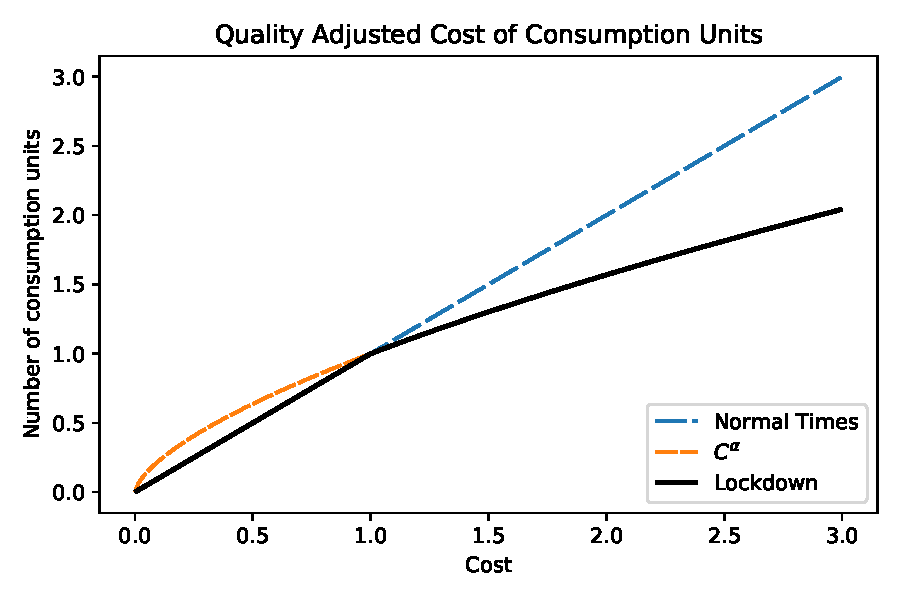
\includegraphics[width=\webWidth\textwidth]{./Figures/QualityCost}
	} %\end{Web}
	{ 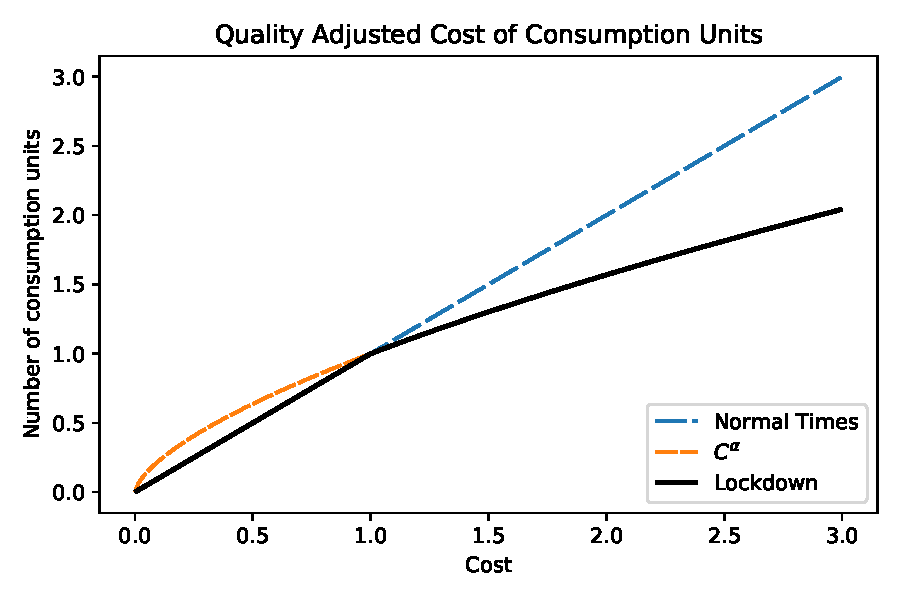
\includegraphics[width=0.8\textwidth]{./Figures/QualityCost}}
\end{figure}

An alternative interpretation is that consumption is made up of a Cobb-Douglass aggregation of two goods:
\begin{eqnarray*}
	C = c_1^{\alpha}c_2^{1-\alpha}
\end{eqnarray*}
During the lockdown, the second good is replaced by home production at a fixed level $\bar{c_2}$. A log-utility function gives $\log(C) = \alpha\log(c_1) + (1-\alpha)\log(\bar{c_2})$, equivalent to our model in which we reduce marginal utility by a factor $\alpha$.



%\processdelayedfloats
\onlyinsubfile{\bibliography{\econtexRoot/LaTeX/ConsumptionResponse}}
\end{document}
% Local Variables:
% TeX-PDF-mode: t
% TeX-command-extra-options: "-output-directory=LaTeX"
% End:
